\documentclass[12pt]{article}

\usepackage[shortlabels]{enumitem}
\usepackage{graphicx}

\begin{document}

\title{Reporte de segunda tarea de Lenguajes de Programaci\'on}
\author{Diego Torres G.}
\date{\today}

\maketitle

\begin{enumerate}
\setcounter{enumi}{4}

		\item{La llamada (bundle '("a" "b" "c") 0) es un buen uso de bundle? ¿qu\'e produce? ¿por qu\'e?}\\\\
				De acuerdo a la definici\'on que usa los procedimientos "take" y "drop", usar $n = 0$, har\'ia que el procedimiento se cicle ya que en cada ocasi\'on se
				har\'ia una llamada recursiva a bundle con los mismos argumentos.\\

				Estar\'ias creando una lista infinita con todos sus elementos siendo listas vac\'ias.\\

				En la implementaci\'on que hay en esta tarea, bundle tira un error con $n = 0$.\\
\setcounter{enumi}{8}
\pagebreak

		\item{Dibuja un diagrama como el de la figura anterior pero para la lista '(11 9 2 18 12 14 4 1).}
				\begin{center}
						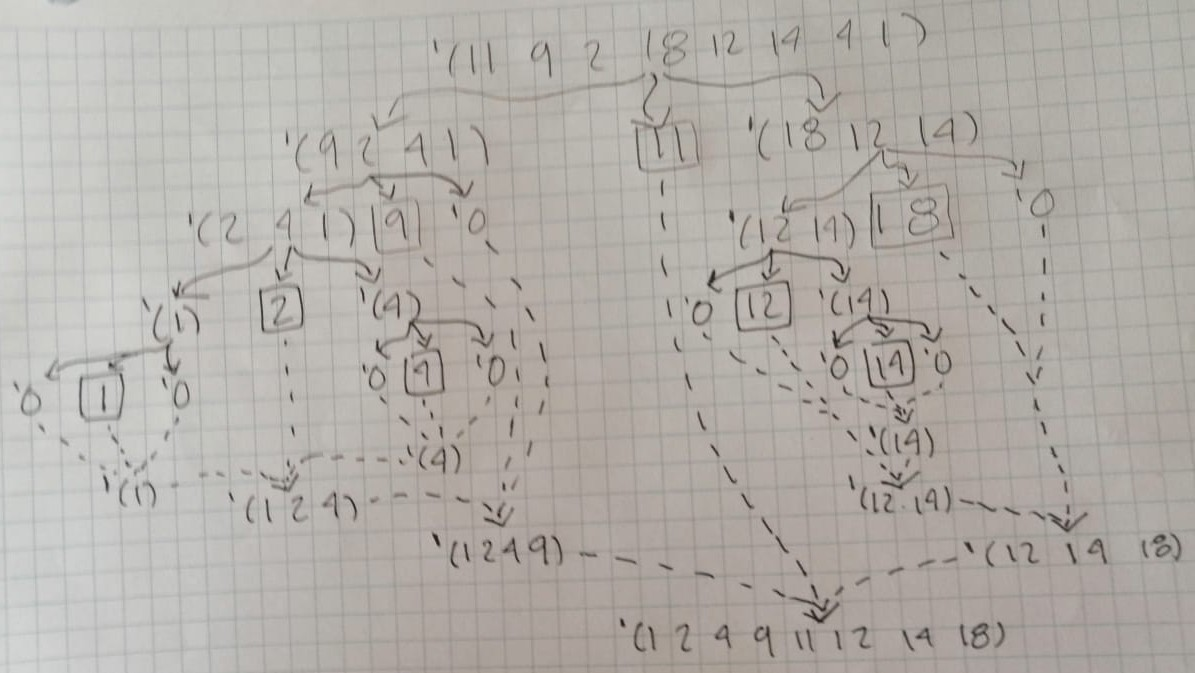
\includegraphics[scale=0.35]{quicksort_diagram.jpeg}
				\end{center}

\setcounter{enumi}{9}

		\item{Implementa los procedimientos smallers y largers.}\\
				De acuerdo a la definici\'on que se ped\'ia, cualquier elemento repetido se quedaba afuera.\\ Decid\'i cambiar el procedimiento largers por 
				larger-or-eq para admitir elementos repetidos.\\ En este caso y con esta implementación, en donde el pivote es el primer elemento, se mantiene la 
				estabilidad del algoritmo.

		\item{Si la entrada a quicksort contiene varias repeticiones de un número, va a regresar una lista estrictamente más corta que la entrada. 
				Responde el por qué y arregla el problema.}\\
				Como mecion\'e en el problema anterior, ya hab\'ia decidido modificar quicksort para aceptar repeticiones en la lista. Esto era porque
				para cada elecci\'on de pivote, se eliminaban las repeticiones de ese elemento al escoger solo los estrictamente mayores o menores.\\

\setcounter{enumi}{12}
		\item{Implementa una versión de quicksort que utilice isort si la longitud de la entrada está por debajo de un umbral. 
				Determina este umbral utilizando la función time, escribe el procedimiento que seguiste para encontrar este umbral.}\\

				Primero, mis supuestos; Tom\'e como si los n\'umeros generados por la funci\'on est\'andar 'random fueran variables independientes e identicamente
				distribuidas, adem\'as, que el tiempo medido por 'time-apply para cada ordenaci\'on no est\'a alterado por ning\'un factor externo de mi computadora
				o de cualquier otro tipo.\\ 
				Todo esto para decir que el tiempo promedio que tomar\'ia a un mismo algoritmo ordenar listas del mismo tama\~no generadas de la misma forma, 
				de acuerdo al teorema de Limite Central, es una variable aleatoria normal.\\

				Teniendo esto en cuenta, hice un procedimiento que mide el tiempo que toma a cada algoritmo ordenar una misma lista y regresa el tama\~no de entrada
				para el cu\'al quicksort es m\'as r\'apido que insertion sort.\\

				Para obtener un tama\~no de lista promedio, hice otro procedimiento que hace n experimentos y 
				calcula el valor esperado para esa muestra de n experimentos.\\

				Finalmente, saqu\'e el valor esperado con 100 experimentos y obtuve como resultado que quicksort es m\'as r\'apido para un tama\~no de entrada de 658
				elementos. Emp\'iricamente, observe que esta variable aleatoria no ten\'ia mucha desviaci\'on y me conform\'e con este n\'umero de experiementos.
				Adem\'as el tiempo que le tom\'o a mi computadora hacer este c\'alculo ya era bastante grande.\\

\end{enumerate}


\end{document}
